% id: 0737
% book: RPM 공통수학2 · 07 명제
% section: 유형 UP 24 절대부등식의 활용
% figure: crop:fig-0737.png
% answer: $20$
% answer_source: 답지
% variant_level: 0 (원본 전사)
% 이 파일은 build.mjs 가 items.json 에서 만든다. 고칠 때는 items.json 을 고친다.
\smash{\raisebox{1.5mm}{\dmkichul{RPM 공통수학2 0737번 · 109쪽}}}
다음 그림과 같이 대각선의 길이가 $2\sqrt{5}$이고 가로, 세로의 길이가 각각 $a$, $b$인 직사각형 모양의 종이를 점선을 따라 접어서 두 밑면이 없는 정사각기둥 모양의 상자를 만들려고 한다. 이 상자의 $12$개의 모서리 길이의 합의 최댓값을 구하시오.
\par\smallskip\begin{center}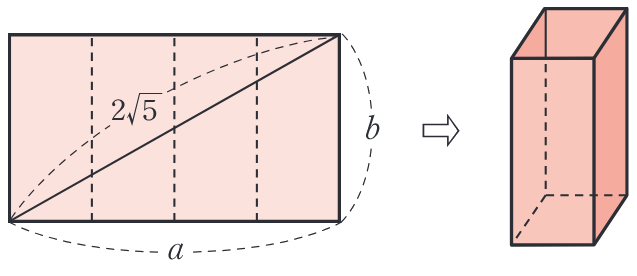
\includegraphics[width=152.6pt]{figures/fig-0737.png}\end{center}
